\section{\textit{Continuum computing}}

\textit{Continuum computing} представља еволуцију претходно поменутих парадигми, интегришући  \textit{edge, fog} и \textit{cloud computing} у један кохезиван динамички систем, трудећи се да усклади локализовани \textit{edge}, средишњи \textit{fog} и централизовани \textit{cloud} пружајући споља кориснику једну јединствену, свеприсутну мрежу уређаја, олакшавајући му коминикацију и интеракцију без потребе за размишљањем о сложености позадинске технологије. Чине га мноштво разноликих уређаја попут мобилних уређаја, сензора и  \textit{IoT} уређаја.

Интегришући ресурсе \textit{cloud}-a, \textit{edge} уређаје и \textit{IoT}, \textit{continuum computing} омогућава ефикасне, \textit{real time} и динамичке рачунске процесе који задовољавају потребе данашњих разноврсних апликација. Он обавља рачунске операције дистрибуирајући оптерећење преко више уређаја у систему. Сваки уређај обавља део посла, а резултати се комбинују како би се произвео крајњи резултат. Ово омогућава брже време обраде и повећану скалабилност. Са \textit{continuum computing}-ом, рачунске операције се ефикасно обављају прилагођавајући се променљивим захтевима и оптимизујући искоришћеност ресурса ван традиционалних граница. Ова алокација ресурса се заснива на факторима као што су близина ресурса, рачунарска способност и давање приоритета задацима који захтевају брзу реакцију. У зависности од задатка, одговори у реалном времену могу бити пренесени на \textit{edge} уређаје, док се комплексна аналитика подразумевано може обавити у \textit{cloud}-у. Ова динамичка дистрибуција задатака побољшава перформансе система и ефикасност обраде док смањује латенцију. Општа архитектура \textit{continuum computing}-а је приказана на слици \ref{fig:continuum_arch}.

\begin{figure}[H]
    \centering
    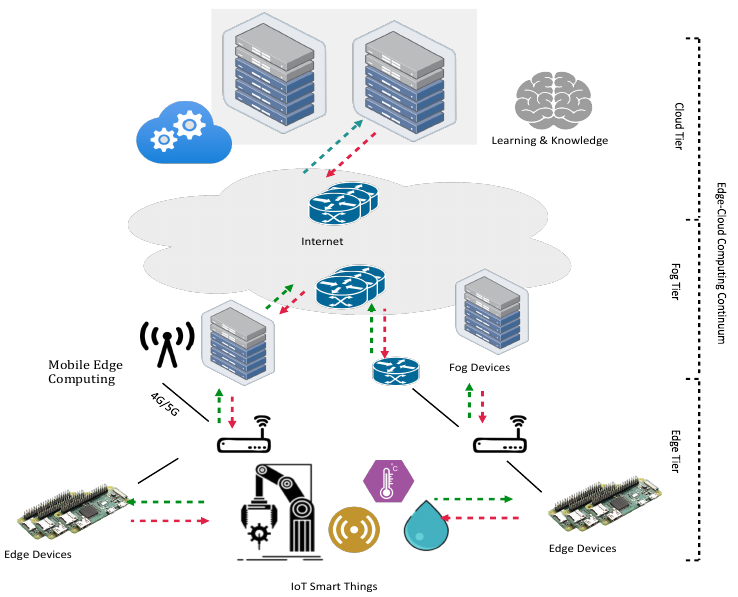
\includegraphics[width=1\textwidth]{images/continuum_arch.png}
    \caption{Архитектура \textit{continuum computing}-а}
    \label{fig:continuum_arch}
\end{figure}

Агилност овакве архитектуре доноси многе предности укључујући  оптимизацију мрежног протока, скалабилност, малу латенцију, ефикасно искоришћене ресурса, балансирање оптерећења, флексибилност и поузданост. Упркос свим овим предностима, наилази се и на одређене потешкоће и изазове као што су међусобна комуникација уређаја различитих произвођача који функционишу служећи се различитим семнатичким правилима, сложеност управљања великог броја уређаја и синхорнизација података.

\pagebreak
\subsection{Могуће примене}

\subsubsection{Паметни градови}

Паметни град користи мрежу сензора и уређаја за прикупљање информација у реалном времену о транспорту, потрошњи енергије, управљању отпадом и јавним услугама. Подаци са ових извора могу се анализирати и користити за донoшење одлука, као средство за повећање комфора, унапређење јавних услуга и квалитет живота грађана. Пошто \textit{continuum computing} има подразумевану скалабилност, он се  може динамички повећавати или смањивати као одговор на промене у екосистему паметног града.

\subsubsection{Здравство}

Здравство обухвата различите медицинске услуге, технологије и системе који су дизајнирани да спрече, дијагностикују, лече и управљају болестима и здравственим стањима. У последњих неколико година развијено је  неколико медицинских уређаја, од мобилних сензора до високопрофесионалних машина (постављених у болницама и здравственим центрима) који се користе за прикупљање података о пацијентима и њихово процесирање путем паметних телефона или у \textit{cloud}-у. Здравствена индустрија захтева тачне и брзе аналитичке резултате од рачунарских уређаја. Понекад је неопходно анализирати захтевне задатке као што су медицински снимци (рентген или ЦТ снимци) или геномско секвенцирање, али се резултат очекује у кратком временском периоду. Понекад је потребно користити вештачку интелигенцију или машинско учење за предвиђање стања пацијента, што захтева више рачунарских ресурса.